
\chapter{Stundenplanung}
\label{chap:schedules}

\section{Manuelle Stundenplanung}

Für die manuelle Planung wird vorerst nur auf die \texttt{Klassenplan Hoch} oder \texttt{Lehrerplan Hoch}-Ansichten eingegangen, weil von der \texttt{Raumplan Hoch} und \texttt{Fachplan Hoch} darf man nichts planen und letzteres liefert ohnehin nur Unfug.\\
\\
Um zu diesen Ansichten zu gelangen klickt man auf den Pfeil nach Unten unter der jeweilige Ressource, dann auf der entsprechende Menüeintrag.

\subsection{Fensterbereiche}

Die Fensterbereiche wurden im allgemeinen im \secref{sec:fensterbereiche}, kurz erläutert. Weil viele wichtige Informationen verteilt über das gesamte Fenster angezeigt werden, wird hier nochmal darauf eingegangen.\\
\\
Der Rasterbereich in Stundenplan-Ansichten ist sowohl für die Darstellung als auch die Gestaltung der Pläne verantwortlich und teilt sich in einen Datum-Bereich, einen Stundenplan-Bereich und einen Bereich für nicht verplante Stunden auf. Im Infobereich stehen Informationen zu der markierte/aktive Block. Sollten Sie noch keinen angeklickt haben, wählt Untis den ersten Block im Stundenplan-Bereich aus.\\
\\
Als Beispiel wird in \figref{fig:klassenplan-hoch-ansicht} ein sehr gefüllter Plan von Fachbereich KMUB dargestellt.

\newpage

\begin{figure}[h]
	\centering
	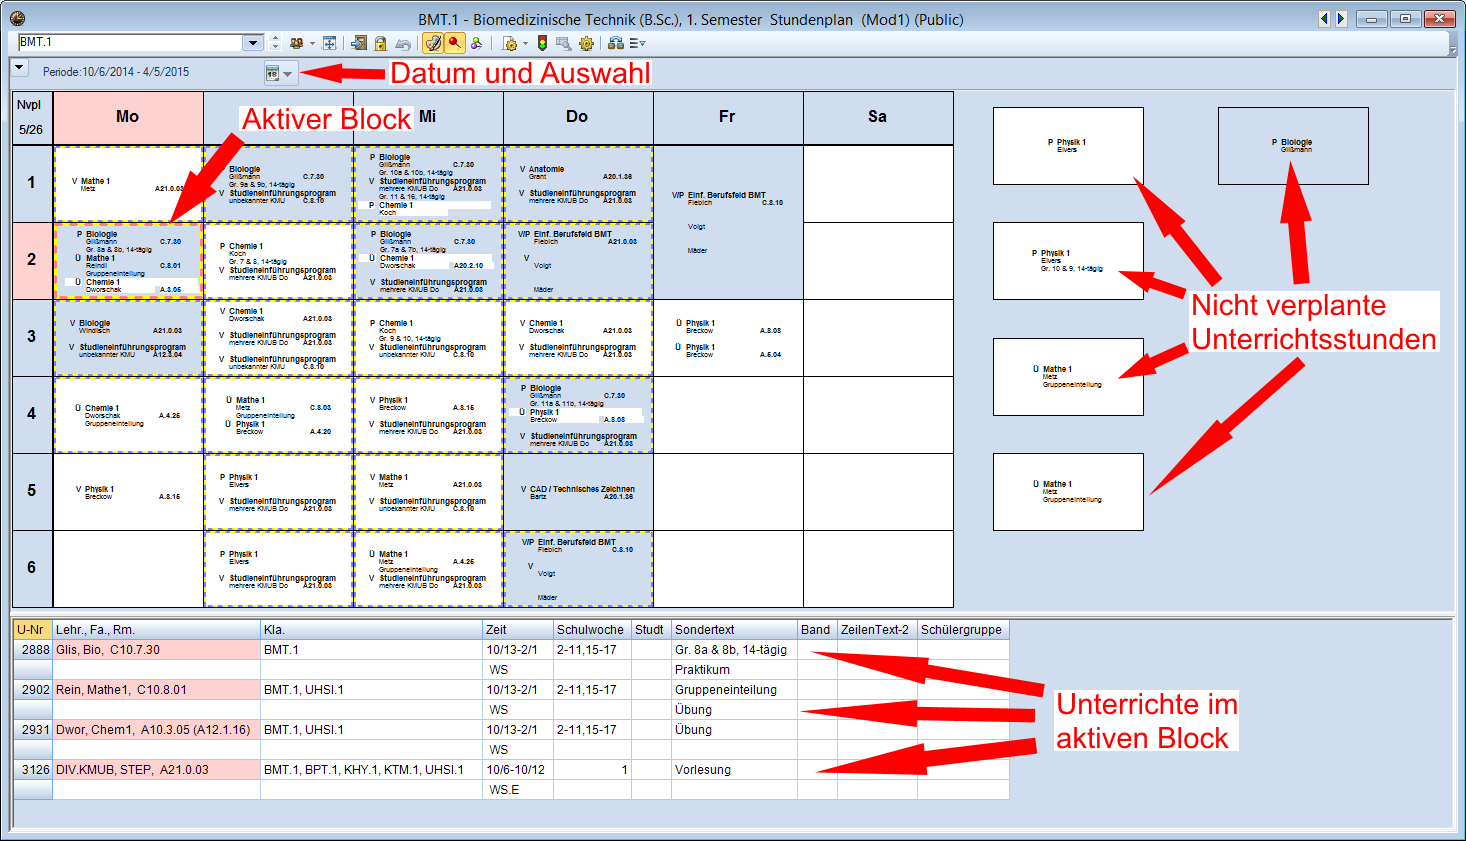
\includegraphics[width=.8\textwidth]{klassenplan-hoch-ansicht}
	\vspace{-5pt}
	\caption{Klassenplan-Hoch-Ansicht}
	\label{fig:klassenplan-hoch-ansicht}
\end{figure}

\subsubsection{Datumbereich}

\begin{wrapfigure}{r}{0.4\textwidth}
	\centering
	\vspace{-14pt}
	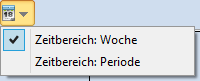
\includegraphics[width=.38\textwidth]{zeitbereich}
	\vspace{-5pt}
	\caption{Zeitbereich Auswahl}
	\label{fig:zeitbereich}
	\vspace{14pt}
	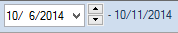
\includegraphics[width=.38\textwidth]{woche}
	\vspace{-5pt}
	\caption{Woche Auswahl}
	\label{fig:woche}
\end{wrapfigure}

Das Datum-Bereich zeigt an für welchen Daten der angezeigte Plan gilt. Man kann zwischen einer Perioden-Darstellung und einer Wochen-Darstellung in dem man das Kalender-Symbol anklickt und den entsprechenden Eintrag auswählt. In \figref{fig:klassenplan-hoch-ansicht}, gilt der angezeigte Plan für das gesamte Wintersemester.\\
\\
Sollte man den Wochen-Ansicht ausgewählt haben werden die Anfangs- und Enddatum der Woche hier dargestellt. Zwischen den beiden Daten gibt es zwei Knöpfe: \UParrow \hspace{2pt} und \DOWNarrow. In dem man auf diese drückt kann man Wochenweise in der Rückwärts \UParrow \hspace{2pt} oder Vorwärts \DOWNarrow \hspace{2pt} durch die Wochen des Schuljahres blättern. In der editierbaren Feld in dem das Startdatum sich befindet kann man auch auf dem $\vee$ klicken um ein Kalender zu öffnen. Mit diesem kann man ggf. Monats- oder gar Jahresweise blättern. Obwohl man die Zahlen des Startdatums bearbeiten kann bewirkt die Änderung diese Angaben nichts.

\subsubsection{Stundenplan-Bereich}

Der Stundenplan-Bereich zeigt die geplanten Stunden abhängig von der ausgewählte Ressource an. Der aktive Block wird mit einer rot \& gelb gefärbten Umrandung angezeigt. Sollte der aktive Block Unterrichte beinhalten werden die andere Stunden dieser mit einem einer blau \& gelb gefärbte Umrandung ebenfalls hervorgehoben.\\

\begin{wrapfigure}{r}{0.3\textwidth}
	\centering
	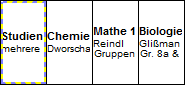
\includegraphics[width=.29\textwidth]{getrennte-unterrichte}
	\vspace{-5pt}
	\caption{Getrennte Darstellung einer Unterrichtsstunde}
	\label{fig:getrennte-unterrichte}
\end{wrapfigure}

\noindent
Die Informationen die Angezeigt werden in der jeweilige Raster Block sind fast beliebig einstellbar und man kann diese Einstellungen speichern damit alles immer so aussieht wie man es braucht. Man sollte unbedingt eine Ansicht speichern in dem alle Unterrichte einer Stunde getrennt angezeigt werden. \figref{fig:getrennte-unterrichte} zeigt ein solche Darstellung der gleichen aktiven Unterrichtsstunde wie in \figref{fig:klassenplan-hoch-ansicht}. Dies ermöglicht die Unterrichte einzeln anzusprechen für Raumzuweisungen, oder um sie zu einem späteren Zeitpunkt einzelnen umplanen zu dürfen. Wenn Stunden so dargestellt werden wie in \figref{fig:klassenplan-hoch-ansicht}, um einen einzelnen Unterricht umplanen zu können, müssten alle vier aus dem Plan gezogen werden und neu verplant werden.\\
\\
Sofern man die Darstellung in Untis nach außen Präsentieren möchte, empfiehlt es sich zwei Stundenplan-Formate zu speichern, wo die zweite nur für die Außendarstellung gedacht ist. Für diesen Zweck ist auch der Plan \figref{fig:klassenplan-hoch-ansicht} gedacht. Es zeigt ein Vielzahl an Informationen ohne durch die Trennung der Unterrichte aufgeteilt zu werden. Mehr dazu \secref{sec:stundenplan-einstellungen}.

\subsubsection{Nicht verplante Stunden}

Im Bereich rechts vom Stundenplan stehen die nicht geplanten Stunden. Bis drei werden die Anzahl an nicht verplanten Stunden eines Unterrichts als Kästchen direkt angezeigt, ab vier wird der Zahl in einem Oval an der obere Kante der Stunden dargestellt.\\
\\
Sollten viele Unterrichte einer Ressource noch nicht verplant sein, kann in diesem Bereich ein ziemliches Durcheinander herrschen. Unter Anderem, können einige Unterrichte soweit nach rechts verschoben sein, dass sie nicht mehr angezeigt werden. Sollte dies der Fall sein, können Sie die angezeigte Unterrichte/Stunden neu gruppieren lassen. Hierzu macht man ein Rechts-Klick irgendwo in diesem Bereich. Ein Kontextmenü erscheint in dem \texttt{N. vpl. Stunden neu gruppieren} als zweite Option erscheint, wählen Sie dieser.

\subsection{Planung}
\label{sec:manuelle-planung}

Die manuelle Stundenplanung geschieht mittels ``Drag \& Drop" Funktionalität. Diese wird anhand \figref{fig:stundenplan-stundenplanung} verdeutlicht. Man zieht dazu eine nicht verplante Stunde von der rechte Seite in einem Block im Stundenplan.\\

\begin{figure}[h]
	\centering
	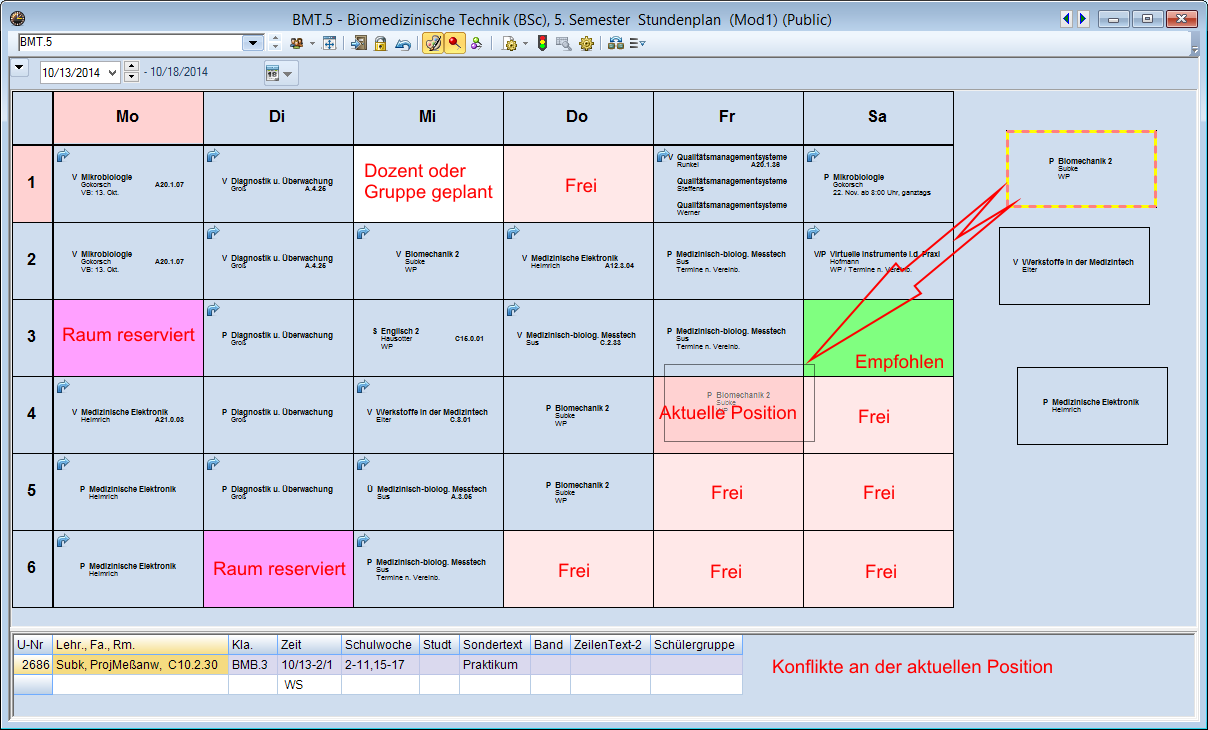
\includegraphics[width=.8\textwidth]{stundenplan-stundenplanung}
	\vspace{-5pt}
	\caption{Manuelle Stundenplanung}
	\label{fig:stundenplan-stundenplanung}
\end{figure}

\noindent
Planungen für die aktuelle Ressource sieht man schon bevor das Ziehen in grau Dargestellt. Sobald man ein solche Stunde über den Stundenplan-Bereich zieht, passen sich die Farben der 'leeren' Stunden die assoziierte Ressourcen dieser Unterrichtsstunde an.\\
\\
Die aktuelle Position der gezogene Stunde wird mit seiner Umrandung und Inhalt angezeigt und der Block, über den er gerade gezogen wird, bekommt ein mittel Rosa Hintergrund-Farbe, wie in \figref{fig:stundenplan-stundenplanung}, Freitag in der 4. Stunde, zu sehen ist. Zusätzlich, sollte ein Ressourcenkonflikt geben in der Stunde, werden konfliktierende Unterrichte im Infobereich eingeblendet. Im \figref{fig:stundenplan-stundenplanung} würde es ein Konflikt wegen Herr Subke, zwischen den zu planenden Block und der Stunde über den sich er gerade gezogen wird, geben.\\
\\
Leere Stunden in dem es Konflikte geben würde werden standardmäßig violett oder weiß gefärbt. Violett entspricht einen Raumkonflikt, wohingegen weiß ein Dozenten- oder Gruppenkonflikt. In \figref{fig:stundenplan-stundenplanung} werden Montag 3. Block und Dienstag 6. violett dargestellt, denn der gewünschte, sprich im Lehrplan enthaltene, Raum (C.8.01) bereits durch andere Veranstaltungen reserviert worden ist. Mittwochs 1. Stunde und Freitags 4. wären weiß dargestellt, denn in die zwei Blöcke ist Herr Subke anderweitig beschäftigt.\\
\\
Stunden die frei sind werden entweder in ein sehr helles rosa oder ein grün Ton dargestellt. Hell rosa ist der normal Zustand einer freien Stunde, grün Töne sind Empfehlungen des Programmes. Im \figref{fig:stundenplan-stundenplanung} sind 8 Stunden noch Konflikt-frei planbar Samstag 3. Stunde wird empfohlen weil es direkt hinter ein geplanter Block liegt und Samstag hat bisher die wenigsten geplanten Stunden.

\subsection{Entplanung}
\label{sec:manuelle-entplanung}

Wenn man die manuelle Planung verstanden hat, ist die Entplanung großteils intuitiv. In fast allen Fällen zieht man einfach die Stunde vom Plan zur rechten Seite. Bei Unterrichte, die mit Wochenstunden versehen sind, ist es auch damit erledigt. Bei Unterrichte die mit Jahresstunden versehen sind ist die Lage etwas kniffliger.\\
\\
Wenn man eine Stunde, die mit Jahresstunden versehen ist, aus dem Stundenplan-Raster zieht, ist nur diese eine Stunde entplant worden. Sollte man mehrere Stunden entplanen wollen gibt es zwei Möglichkeiten. Hat man die Ansicht so eingestellt, dass Unterrichte im Plan im Fall einer Kollision getrennt dargestellt werden und alle zusammenhängende Unterrichtsstunden als eine Einheit dargestellt werden, kann man diese zusammenhängende Unterrichtsstunden auf einmal vom Stundenplan ziehen. Man kann auch die Anzahl der Stunden reduzieren oder auf null setzen. Bei einer Reduzierung der Stunden werden, zeitlich gesehen, Stunden von hinten nach vorne entplant, d.h. Stunden die später im Schuljahr stattfinden werden eher entplant. Bspw. wenn Unterrichtsstunden in die zweite und dritte Januar Woche, sowie in der erste Woche April, werden erst die Unterrichtsstunden in April entplant, dann die Stunden in der dritte Januar Woche, dann im zweiten. Bei einer Reduzierung auf null, werden entsprechend alle Unterrichtsstunden entplant.\\
\\
Was, die Entplanung von sporadische Unterrichtsstunden verkompliziert, ist, dass Untis davon ausgeht, dass man manuell entplante Stunden noch in der selben Woche stattfinden lassen möchte. D.h. die entplante Stunde ist normalerweise an der Woche in der sie entplant war gebunden. Man kann diese Wochenverbindung umgehen in dem man die \texttt{STRG}-Taste hält bevor man die Stunde oder Stunden aus dem Raster zieht.

\section{Planungsdialog}

Diese Sektion wird als letztes gepflegt.

\section{Automatisierte/Optimierte Planung}

Diese Planungsmöglichkeit werde ich im Frühling angehen.












